	\chapter{Detecting \ac{EWFO} on \ac{MAV}}
	\label{sec:object_detection}
	
	\ac{CNN}-based Object Detectors offer the advantage that they can be trained on any object given labelled training data is available. However, typically the architectures of \acp{CNN} are optimized for solid feature rich objects, such as planes, cars or faces. The predominant metrics optimized are precision and recall rather than inference speed. This work investigates the detection of \ac{EWFO} on \acp{MAV} as part of a control loop. Hence, inference speed and computational requirements can be more important than detection performance. Furthermore, \acp{EWFO} differ substantially from objects usually used in Object Detection. This chapter investigates the detection of \acp{EWFO} with a \acp{CNN}. An off-the-shelve \acp{CNN}-based detector is optimized for the detection of \acp{EWFO}. Furthermore, the trade-off in detection performance and inference speed is studied in the example of the hardware used in this thesis. The research questions are summarized in the following:
	
\begin{enumerate}
	\item[\textbf{RQ2}]How can the architecture be optimized to detect \acp{EWFO} more efficiently?
	\item[\textbf{RQ3}]What are the trade-offs in detection performance and inference time when the detection model for \acp{EWFO} is deployed on a \ac{MAV}?
%	\item[\textbf{RQ4}]Can the gained insights be used to build a lightweight and robust detection model for racing gates in the \ac{IROS} Autonomous Drone Race?
\end{enumerate}

	\section{Methodology}
		
	This work uses the TinyYoloV3 model as baseline. The model is implemented using \textit{keras} with \textit{tensorflow} backend. In the following the architecture and training goal are summarized.
	
	\subsection{Training Goal}
	The original training goal is defined as follows:
	\if false
	\begin{align}
	&\lambda_{coord} \sum_{i=0}^{S^2}\sum_{j=0}^B \mathbb{1}_{ij}^{obj}[(x_i-\hat{x}_i)^2 + (y_i-\hat{y}_i)^2 ] \\&+ \lambda_{coord} \sum_{i=0}^{S^2}\sum_{j=0}^B \mathbb{1}_{ij}^{obj}[(\sqrt{w_i}-\sqrt{\hat{w}_i})^2 +(\sqrt{h_i}-\sqrt{\hat{h}_i})^2 ]\\
	&+ \sum_{i=0}^{S^2}\sum_{j=0}^B \mathbb{1}_{ij}^{obj}(C_i - \hat{C}_i)^2 + \lambda_{noobj}\sum_{i=0}^{S^2}\sum_{j=0}^B \mathbb{1}_{ij}^{noobj}(C_i - \hat{C}_i)^2 \\
	&+ \sum_{i=0}^{S^2} \mathbb{1}_{i}^{obj}\sum_{c \in classes}(p_i(c) - \hat{p}_i(c))^2 \\
	\end{align}
	\fi
	
	\begin{equation}
	\mathcal{L} = \lambda_{loc}\mathcal{L}_{loc} + \lambda_{obj}\mathcal{L}_{obj} + \lambda_{noobj}\mathcal{L}_{noobj} + \lambda_{class}\mathcal{L}_{class}
	\end{equation}
	where $\mathcal{L}_{loc}$ is the target for bounding box regression, $\mathcal{L}_{obj}$ the loss where a object is present, $\mathcal{L}_{noobj}$ the loss where there is no object and $\mathcal{L}_{class}$ the classification loss. $\lambda$ are trade-off parameters between the multiple targets.
	
	For a single class prediction this can be simplified to:
	
	\begin{equation}
	\mathcal{L} = \lambda_{loc}\mathcal{L}_{loc} + \lambda_{obj}\mathcal{L}_{obj} + \lambda_{noobj}\mathcal{L}_{noobj}
	\end{equation}
	
	The object loss is defined as:
	
	\begin{equation}
		\mathcal{L}_{obj} = \sum_{i=0}^{S^2}\sum_{j=0}^B \mathbb{1}_{ij}^{obj}(-(c_{ij}\log(\hat c_{ij}) + (1 - c_{ij})\log(1 - \hat c_{ij})))
	\end{equation}
	where $\hat c_{ij}$ is an output node with softmax activation assigned to anchor box $i$,$j$, $ c_{ij}$ the ground truth label assigned to that box, 1 for an object and 0 for no object.  $\mathbb{1}_{ij}^{obj}$ is 1 if the anchor box at $i$,$j$ is responsible to predict a certain object and 0 otherwise. The responsibility is determined by \ac{IoU} with a ground truth box. The box with the highest \ac{IoU} with the ground truth box gets assigned responsible.
	
	$\mathcal{L}_{obj}$ is defined vice versa but triggered by the $\mathbb{1}_{ij}^{noobj}$ binary variable.

	The localization target is defined as:
	
	\begin{equation}
		\mathcal{L}_{loc} = \sum_{i=0}^{S^2}\sum_{j=0}^B \mathbb{1}_{ij}^{obj}[(x_{ij}-\hat{x}_{ij})^2 + (y_i-\hat{y}_{ij})^2  + (\sqrt{w_{ij}}-\sqrt{\hat{w}_{ij}})^2 +(\sqrt{h_{ij}}-\sqrt{\hat{h}_{ij}})^2 ]
	\end{equation}
	where $x_{ij}$,$y_{ij}$ are the ground truth center coordinates of anchor box $i,j$ and $w_{ij}$,$h_{ij}$ the corresponding width and height. $\hat x_{ij}$,$\hat y_{ij}, \hat w_{ij}$,$\hat h_{ij}$ are the predicted bounding box coordinates. $\mathbb{1}_{ij}^{obj}$ is 1 if the set of output nodes at $i$,$j$ is responsible to predict a certain object and 0 otherwise. 
	
	\subsection{Baseline Architecture}
	
	\Cref{fig:tinyyolov3_arch} shows the a diagram of the baseline TinyYoloV3- architecture. The input image of 416x416 is processed by 5 common layers that decrease the spatial resolution stepwise (max pooling) down to 26x26. Thereby the number of filters per layer increases up to 512. From layer 5 the network splits to two branches responsible for smaller and larger objects. The lower branch predicts larger objects at a grid of 13x13. The higher branch predicts smaller objects at a grid of 26x26.
	
	\begin{figure}[hbtp]
			\centering
		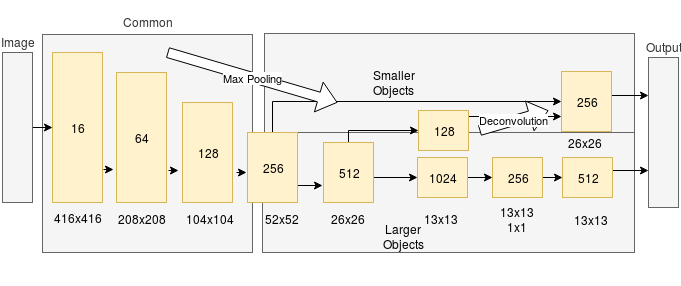
\includegraphics[width=0.8\textwidth]{fig/tinyyolov3_arch}
		\caption{The architecture of the baseline TinyYoloV3. In the common part the spatial resolution decreases each layer down to 26x26, while the width increases from 16 to 512. From layer 5 two branches focus on objects corresponding to different scales. }
		\label{fig:tinyyolov3_arch}
	\end{figure}

	\subsection{Datasets}
	
	Throughout the experiments the same training and test set is used. For training 20 000 samples from the dataset created in \Cref{sec:datagen} are used. For testing we use the test set described in \Cref{sec:datagen:method}.

	For all trainings the Adam optimizer is applied using a learning rate of 0.001 for the first 60 epochs and a learning rate 0.0001 afterwards. A validation set containing 1\% randomly sampled images from the training set is used. The training is stopped if the validation error does not decrease for more than 5 epochs or 100 epochs are reached.
	
	\section{Depth and Width}
	
	State of the art results of Computer Vision benchmarks are achieved by particularly deep/wide models. The vast amount of parameters and layers enables to model highly non-linear functions and complex image features. However, \acp{EWFO} do not contain particularly complex shapes. Instead the object parts are of thin structure and are spread across large parts of the image. Hence, we hypothesize that a very deep/wide network will not perform better than a shallower and thinner counterpart. Also, the baseline architecture is designed to detect complex objects of multiple classes. In this work we investigate the single class case. We hypothesize that this requires less filters and thus that a thinner and shallower counterpart can detect the object with equal performance.
	
	\subsection{Experiment}
	
	In order to evaluate our hypothesis an experiment is conducted. The network is trained with different architectures and the performance is evaluated. In a first experiment the TinyYoloV3 architecture is used as baseline and the number of filters is decreased stepwise by a factor of 2. The number of layers is held constant. In a second experiment the width is held constant and the depth is varied. The exact scheme to change depth is visualized in \Cref{fig:depth_changes}. In order to remove layers the convolutional layers are removed while the pooling layers are kept. For the increase of depth 2 layers are inserted stepwise at the end of both branches.  
	
		\begin{figure}[hbtp]
			\centering
			\includegraphics[width=0.8\textwidth]{fig/depth_changes}
			\caption{Architectural Changes when varying the depth. The upper graph shows in which order layers are removed. The lower graph shows how layers are added. Depth is increased by inserting two layers on each branch (green). }
			\label{fig:depth_changes}
		\end{figure}
	
	\subsection{Results}
	
	\Cref{fig:perf_width} shows the performance for thinner and wider networks. It is apparent how the performance only undergoes slight variations despite reducing the total number of weights by a factor 1000. \todo{retrain one in the middle to get variance, it should be more linear}
	
	
	\begin{figure}[hbtp]
		\centering
		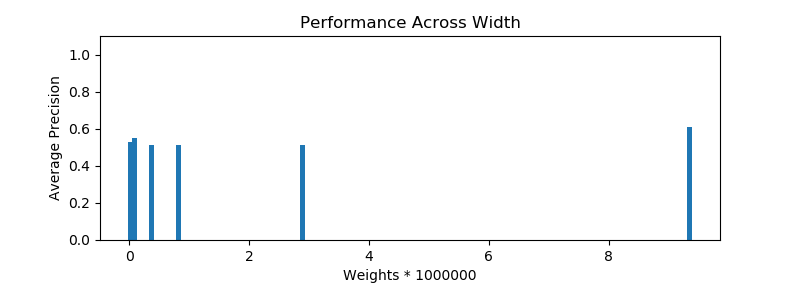
\includegraphics[width=\textwidth]{fig/perf_width}
		\caption{Performance in simulation when varying the amount of filters per layer. Starting from the baseline architecture with approximately 9 Mio. weights, the amount of filters per layer are decreased stepwise by a factor of 2. Only minor effects on performance can be seen, despite reducing the flexibility of the model.}
		\label{fig:perf_width}
	\end{figure}
	
	\Cref{fig:perf_depth} shows the performance for different amount of layers. It can be seen how the performance increases significantly up to a depth of 8. Further increase in depth does not lead to better overall performance. However, depth has a larger influence on the performance for different object sizes as displayed in \Cref{fig:depth_ap_size}. It can be seen how the deeper models perform better at larger object sizes. The deepest model however looses performance for the smaller object sizes.

	\begin{figure}[hbtp]
		\centering
		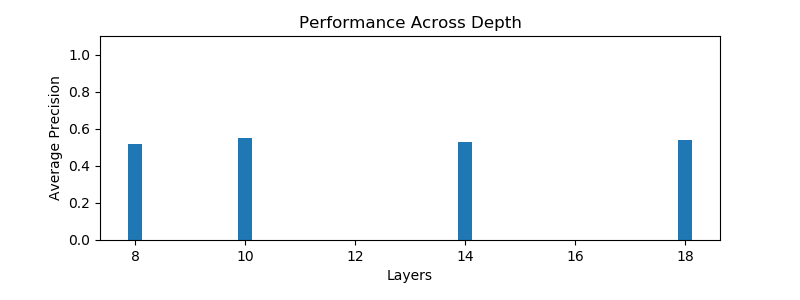
\includegraphics[width=\textwidth]{fig/perf_depth}
		\caption{Performance in simulation when varying the amount of layers. The exact architectures are shown in \Cref{fig:depth_changes}. The overall performance does not increase further with more than 8 layers.}
		\label{fig:perf_depth}
	\end{figure}


	\begin{figure}[hbtp]
		\centering
		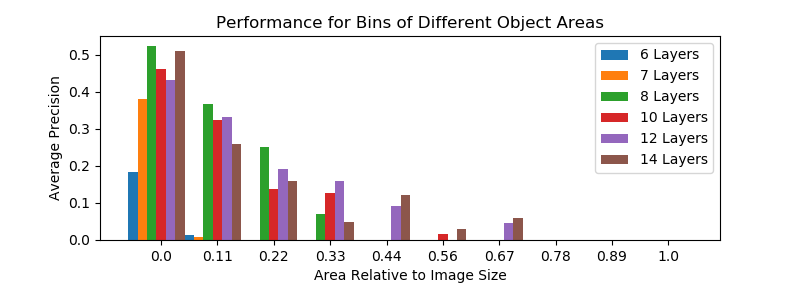
\includegraphics[width=\textwidth]{fig/depth_ap_size}
		\caption{Performance in simulation of models with varying depth and for bins of different size. It can be seen that the performance for larger objects increases with the amount of layers.}
		\label{fig:depth_ap_size}
	\end{figure}
	
	\Cref{fig:size_bins} shows the distribution of object sizes in the bins used for evaluation. It can be seen that most objects in the test set are further away. \todo{put some examples to show what each size actuall means}
	
	\begin{figure}[hbtp]
		\centering
		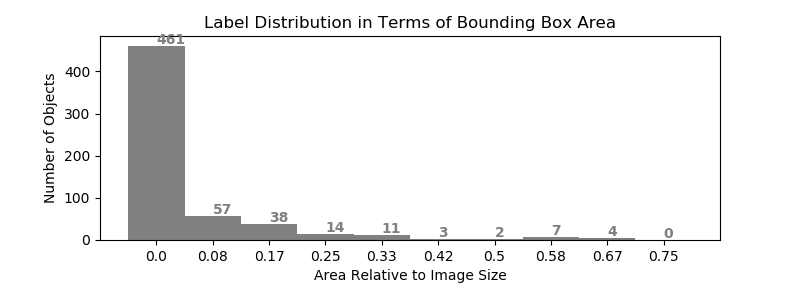
\includegraphics[width=\textwidth]{fig/distr_size}
		\caption{Label distribution in bins of different object size. As the field of view is larger for objects further away, the proportion of small objects is higher.}
		\label{fig:size_bins}
	\end{figure}
	
	\subsection{Discussion}
	
	The overall performance is only slightly affected when reducing the number of weights in terms of width and height. We can assume that this is because the objects we investigate are of quite simple structure. Intuitively the features to be considered are color, lines and edges in certain combinations. Hence, it seems logical that only a few filters are necessary to represent these shapes.
	
	The performance in terms of different object sizes varies significantly for models with varying depth. Only deeper networks are able to detect larger objects. However, the complexity of the object does not increase for closer objects. In contrary the closer the objects are, the less context is visible. A very close object consists "only" of an orange square. Hence, it is unlikely that increased flexibility is the reason for the increase in performance. 
	
	Instead it is more likely that the increased receptive field is the reason for the improved performance. In fact only the network with 14 layers has a receptive field of 414 an thus covers the whole image. Yet even this network cannot detect the largest objects. Thus the receptive field can not be the only reason for the lower performance on larger objects.
	
	 The current structure combines features distributed across space in a pyramid fashion. So 3-by-3 convolutions are performed layer by layer such until the whole image is covered. For \acp{EWFO} many of these steps are unnecessary as the objects are empty and the network should learn to ignore the empty part in the centre. It is possible that this structure gets confused by the parts that are present in the image centre.
	
	\subsection{Conclusion}
	
	We investigated how width affects the performance for the detection of \acp{EWFO}. We hypothesized that due to the low variance in the investigated object and the simple features, less filters are required than in the baseline architecture. We can confirm this hypothesis as we see that the width can be decreased by a factor of 10 without loosing performance. This leads to a reduction of weights by a factor of 1000. 
	
	Furthermore, we investigated how depth affects the performance of the model. We hypothesized that a shallow network should be able to detect the object as it only consists of relatively simple features. We can see how depth is required in order to cover the whole input image. Hence, we cannot fully conclude whether depth is required for the increased flexibility or simply due to the receptive field. 
	
	\section{Receptive Field}
	
	In shallow fully convolutional networks the receptive field of the last layer might not cover the whole image. This is of particular effect for \ac{EWFO} as thus it is possible that the output layer which gets assigned responsible to predict the object does not see any feature of its parts.
	
	A deeper network is one way to increase receptive field but comes at cost of computation. In this section we investigate whether the same performance can be reached by using alternative ways to increase the receptive field.
	
	\subsection{Experiment}
	
	 A 7-by-7 max-pooling layer is inserted on the lower branch after layer 6. The model is compared to the architecture with 14 layers and a model where we replace the 3-by-3 kernel of layer 6 with a 9-by-9 kernel.
	 
	 \subsection{Results}
	 
	\section{Anchors and Output Grid}
		
	\section{Reducing Inference Time}
	
	To this end we investigated how to incorporate 
	Next to performance, inference time is a crucial parameter for the detection of \ac{EWFO} on \ac{MAV}. 
	
	 It is determined by the number of computations but also how these computations can be executed. Theoretically the convolutions of one layer in a \acp{CNN} can be executed fully in parallel, however this operation has to be supported by the computational platform. The execution time further depends on how fast a computational platform can execute multiplications, how large the memory is and how fast it can be accessed, but also on the particular low level software implementation. So far we created a model that is 
	 
	 \section{What did we learn?}
	
	\section{Implementation on the \ac{MAV}}